\documentclass[12pt]{article}
\usepackage[utf8]{inputenc}
\usepackage[spanish, ]{babel}
\decimalpoint
\usepackage{amsmath}
\usepackage{amsfonts}
\usepackage{amssymb}
\usepackage{minted}
\usepackage{amsthm}
\usepackage{hyperref}
\hypersetup{
  % hidelinks = true,   % Oculta todos los enlaces.
  colorlinks = true,   % Muestra todos los enlaces, sin bordes alrededor.
  linkcolor={magenta},     % Color de enlaces genéricos
  citecolor={blue!70!black},   % Color de enlaces de referencias
  urlcolor={blue!70!black}     % Color de enlaces de URL
}

\title{Métodos Avanzados en Estadística \\ \Large{Ejercicios Bootstrap}}
\author{Antonio Coín Castro}
\date{\today}

\usepackage{natbib}
\usepackage{graphicx}
\usepackage{physics}
\usepackage{subfigure}
\usepackage{enumitem}

\renewcommand{\phi}{\varphi}
\renewcommand{\epsilon}{\varepsilon}
\newcommand{\md}[1]{\left|#1\right|}
\newcommand{\C}{\mathbb{C}}
\newcommand{\R}{\mathbb{R}}
\newcommand{\N}{\mathbb{N}}
\newcommand{\I}{\mathbb{I}}

\newcommand\restr[2]{{% we make the whole thing an ordinary symbol
  \left.\kern-\nulldelimiterspace % automatically resize the bar with \right
  #1 % the function
  \vphantom{\big|} % pretend it's a little taller at normal size
  \right|_{#2} % this is the delimiter
  }}

\usepackage[left=2.25cm, right=2.25cm, top=2.25cm, bottom=3.00cm]{geometry}

\newcommand\numberthis{\addtocounter{equation}{1}\tag{\theequation}}
\newenvironment{resol}{\textbf{Resolución.}}{\qed}
\newtheorem{ejer}{Ejercicio}%[section]
\newtheorem{subejer}{Apartado}[ejer]

\begin{document}
\maketitle

\begin{ejer}
Se extrae una remuestra bootstrap de una muestra de $n$ observaciones $X_1,\dots,X_n$. Calcula la probabilidad de que una observación prefijada, $X_j$, no aparezca en la muestra bootstrap. Calcula el límite de esta probabilidad si $n\to \infty$.
\end{ejer}

\textit{Solución.} En primer lugar, llamemos $n_j$ al tamaño del conjunto $\{i: X_i = X_j\}$ tras la observación original ($1 \leq n_j \leq n$). Sabemos que la función de distribución empírica representa una distribución que asigna probabilidades de $1/n$ a cada observación de la muestra original. Por tanto, la probabilidad de que al muestrear la distribución empírica una única vez no obtengamos la variable $X_j$ es de $1- n_j/n$. Así, se tiene:

\[
p^n_j = P(X_j \notin \{X_1,\dots, X_n\}) = P(X_j \neq X_1 \land \dots \land X_j \neq X_n) = \left( 1 - \frac{n_j}{n}\right)^n.
\]
Tomando límite cuando $n\to\infty$ llegamos a que

\[
\lim_{n\to\infty} p^n_j = \lim_{n\to\infty}  \left( 1 - \frac{n_j}{n}\right)^n = e^{-n_j}.
\]

Si suponemos que todas las observaciones son diferentes, $n_j=1$ para todo $j$, y tenemos que el límite de la probabilidad buscada vale $1/e$. Dicho de otra forma, para un número grande de observaciones, la fracción esperada de datos originales que no son seleccionados en cada remuestra bootstrap es de $1/e \approx 0.368$.

\begin{ejer}
Dada una muestra de $n$ datos diferentes, calcula en función de $n$ el número de remuestras bootstrap distintas que es posible obtener. Aplica la expresión obtenida al caso $n=15$. ¿Qué implicaciones tiene el resultado?
\end{ejer}

\textit{Solución}. El número total de remuestras bootstrap que podemos obtener serán las \textit{combinaciones con repetición} de $n$ elementos, tomadas de $n$ en $n$. Es decir, las posibles formas de elegir $n$ elementos (cada una de las remuestras bootstrap individuales) de un conjunto de $n$ elementos distintos (los datos originales), donde no importa el orden y se pueden repetir los elementos. Sabemos que este número es:

\[
\begin{pmatrix}
  2n -1\\
  n
\end{pmatrix} = \frac{(2n-1)!}{n!(n-1)!}.
\]

Si aplicamos esta fórmula al caso $n=15$ obtenemos que el número de remuestras bootstrap distintas que podemos obtener a partir de una muestra de 15 datos diferentes es:

\[
\begin{pmatrix}
  29\\
  15
\end{pmatrix} = \frac{29!}{15!\cdot 14!} \approx 7.76 \cdot 10^{7}.
\]
Es decir, el espacio de búsqueda tendría un tamaño de casi 80 millones de puntos de dimensión $n$. La consecuencia de este resultado es que incluso para tamaños de muestras pequeños no es factible calcular de forma exacta la distribución de los estimadores bootstrap, pues rápidamente excedemos la capacidad de cómputo de los ordenadores actuales. Nos conformamos con hacer estimaciones de Monte Carlo de estos estimadores, hasta un tamaño $B$ elevado pero factible.


\begin{ejer}
Consideremos la siguiente muestra de tamaño $n=10$:
\[
1 \quad 2 \quad 3.5 \quad 4 \quad 7 \quad 7.3 \quad 8.6 \quad 12.4 \quad 13.8 \quad 18.1
\]
Sea $\hat\theta$ la media recortada al 40\% que se obtiene al eliminar los dos mayores y los dos menores datos y calcular el promedio de los 6 datos restantes. Sea $\hat\sigma_R$ el estimador bootstrap de la desviación típica de $\hat\theta$ basado en $R$ remuestras. Calcula $\hat\sigma_R$ para $R=10,100,1000,2000$ y usando 10 conjuntos independientes de $R$ remuestras. ¿A qué valor parecen converger los valores obtenidos? ¿Qué número de remuestras te parece suficiente?
\end{ejer}

\textit{Solución.} Consideramos el caso general para muestras de tamaño $n$, donde $\hat\theta$ es la media recortada (aproximadamente) al tanto por 1 dado por $q$, de forma que se recortan $k = \lfloor qn/2 \rfloor$ elementos de cada extremo de la muestra ordenada. Sabemos que en este caso el estimador bootstrap ideal de la varianza es

\[
Var_{F_n}(\hat\theta^*)=E_{F_n}\left[\left(\hat\theta^{*}-E_{F_n}[\hat\theta^*]\right)^2\right],
\]
que a su vez aproximamos mediante $R$ remuestras bootstrap por

\begin{equation}
  \label{eq:bootstrap}
\hat\sigma_R^2 = \frac{1}{R-1}\sum_{j=1}^R \left(\hat\theta_j^{*}- \bar\theta^*\right)^2,
\end{equation}
donde $\hat\theta^*_j$ es el valor del estimador para la remuestra $j$ y $\bar\theta^*=R^{-1}\sum_{j=1}^R \hat\theta^*_j$ es el promedio de todas las versiones bootstrap. Concretamente, si $X_{(1)}^{*j}, \dots, X_{(n)}^{*j}$ es la remuestra $j$-ésima ordenada, se tiene que

\[
\hat\theta^*_j = \frac{1}{n-2k} \sum_{i=k+1}^{n-k} X_{(i)}^{*j}.
\]

Así pues, nuestro estimador bootstrap es $\hat\sigma_R=\sqrt{\hat\sigma_R^2}$. Para calcularlo con distintos valores de $R$ escribimos un programa. En primer lugar, definimos los parámetros del problema:

\begin{minted}{R}
library(ggplot2)
set.seed(42)

Rs <- c(10, 100, 1000, 2000)
nrep <- 500
sample_orig <- c(1, 2, 3.5, 4, 7, 7.3, 8.6, 12.4, 13.8, 18.1)
n <- length(sample_orig)
q <- 0.4
\end{minted}

El cuerpo de nuestro programa seguirá la siguiente secuencia lógica: para cada valor de $R$ realizamos \verb|nrep| repeticiones independientes de la estimación bootstrap, y guardamos los resultados de la desviación típica estimada de la media recortada para realizar posteriormente un histograma.

\begin{minted}{R}
for (R in Rs) {
  sd_trimmed_mean <- vector(, nrep)

  for (i in 1:nrep) {
    # Generate R bootstrap resamples of size n (n x R matrix)
    resample_bootstrap <- sample(sample_orig, n * R, rep = T)
    resample_bootstrap <- matrix(resample_bootstrap, nrow = n)

    # Sort the columns in ascending order
    resample_bootstrap <- apply(resample_bootstrap, 2, sort, decreasing = F)

    # Trimmed mean of each bootstrap resample
    trimmed_mean_bootstrap <- apply(resample_bootstrap, 2, mean, trim = q/2)

    # Bootstrap estimator of the standard deviation of the trimmed means
    sd_trimmed_mean[i] <- sd(trimmed_mean_bootstrap)
  }

  # Histogram and estimated density of the bootstrap estimates
  df <- data.frame(sd_trimmed_mean = sd_trimmed_mean)
  p <- ggplot(df, aes(x=sd_trimmed_mean)) +
    geom_histogram(aes(y =..density..),
                   bins = 30, fill = "#69b3a2", col = 'black') +
    geom_density(aes(y=..density..)) +
    ggtitle(paste("R =", R))
  print(p)
}
\end{minted}

Los resultados obtenidos podemos verlos en la siguiente figura. Como vemos, el valor estimado $\hat\sigma_R$ oscila en torno a 2, y para valores más grandes de $R$ parece estabilizarse entre $2$ y $2.05$, reduciendo su varianza. Un valor suficiente de $R$ para llegar a esta conclusión podría estar entre 100 y 1000, donde la variación es ya lo suficientemente pequeña.

\begin{figure}[h!]
\centering
\subfigure{
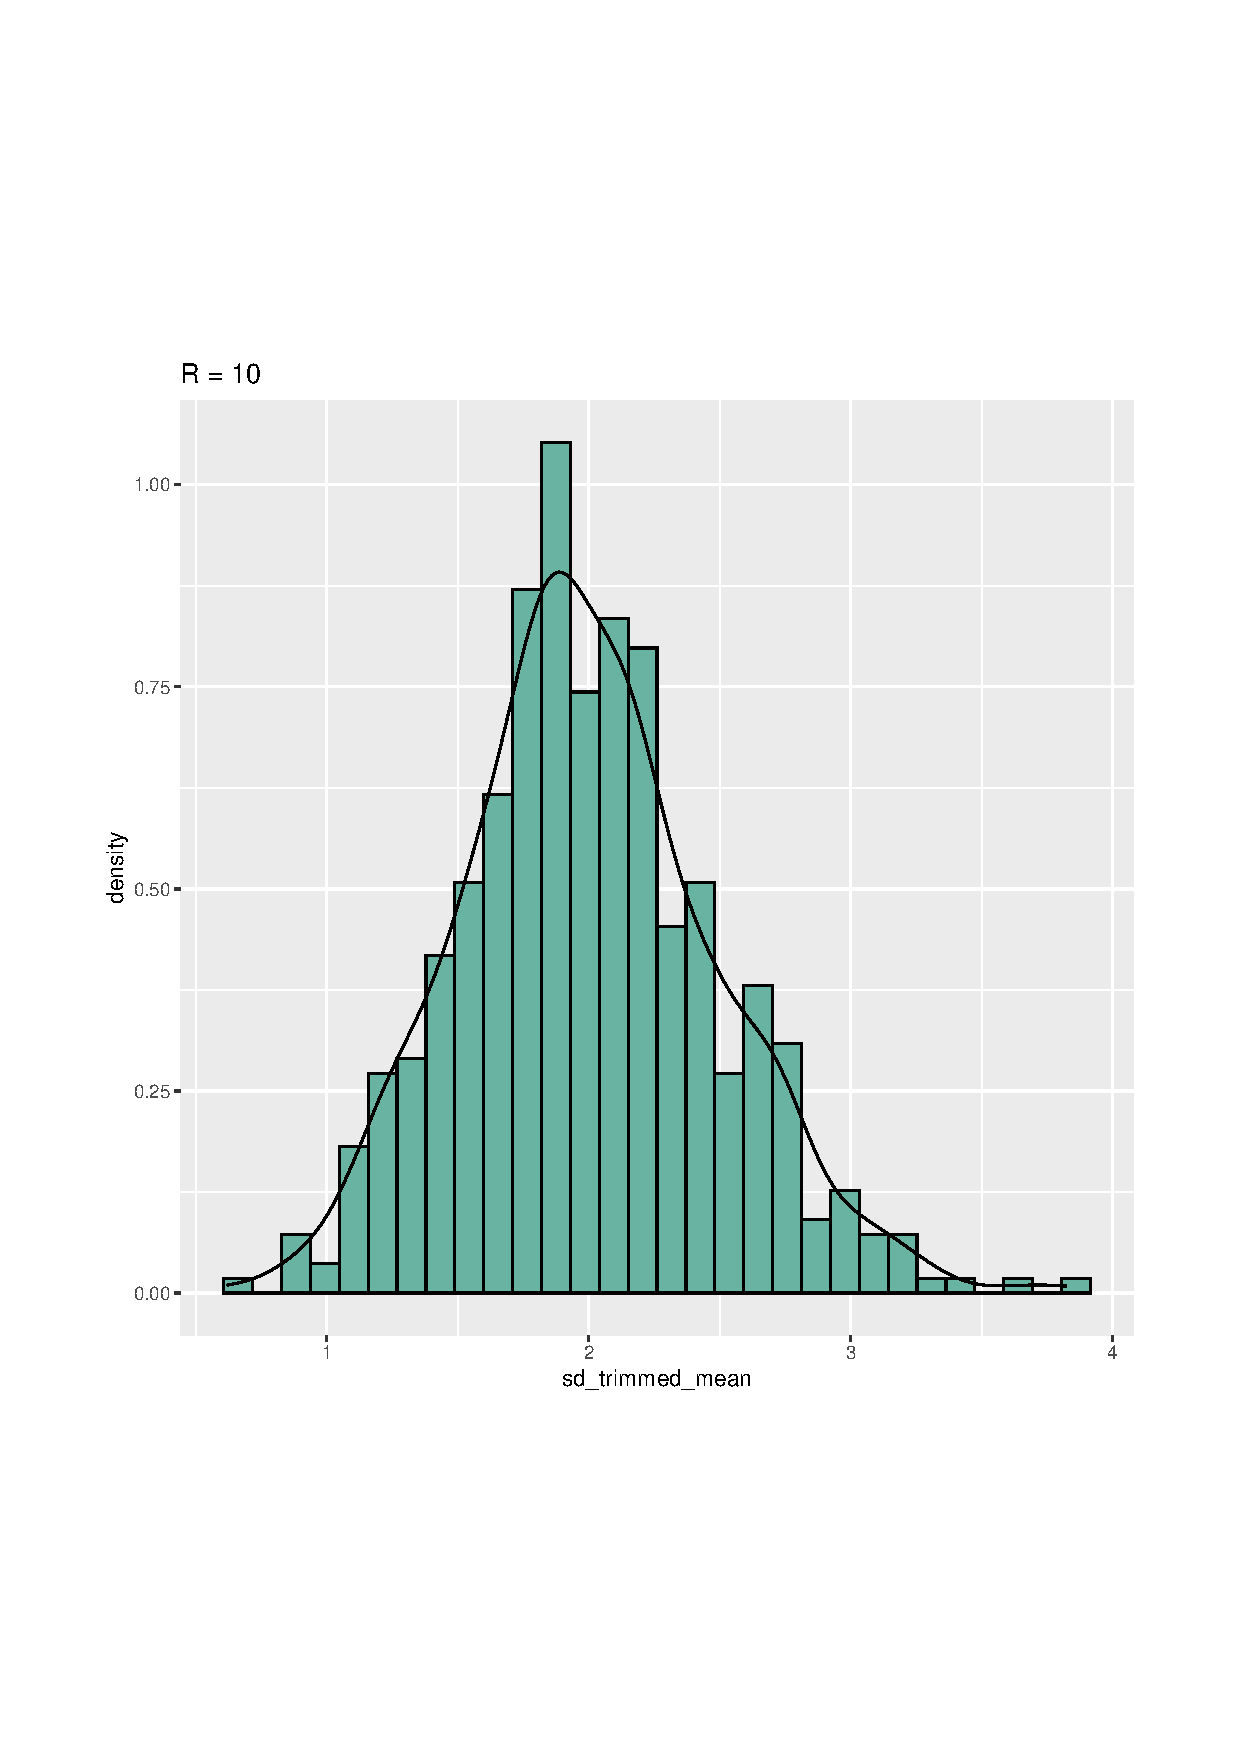
\includegraphics[width=.45\textwidth]{img/fig1}
}
\subfigure{
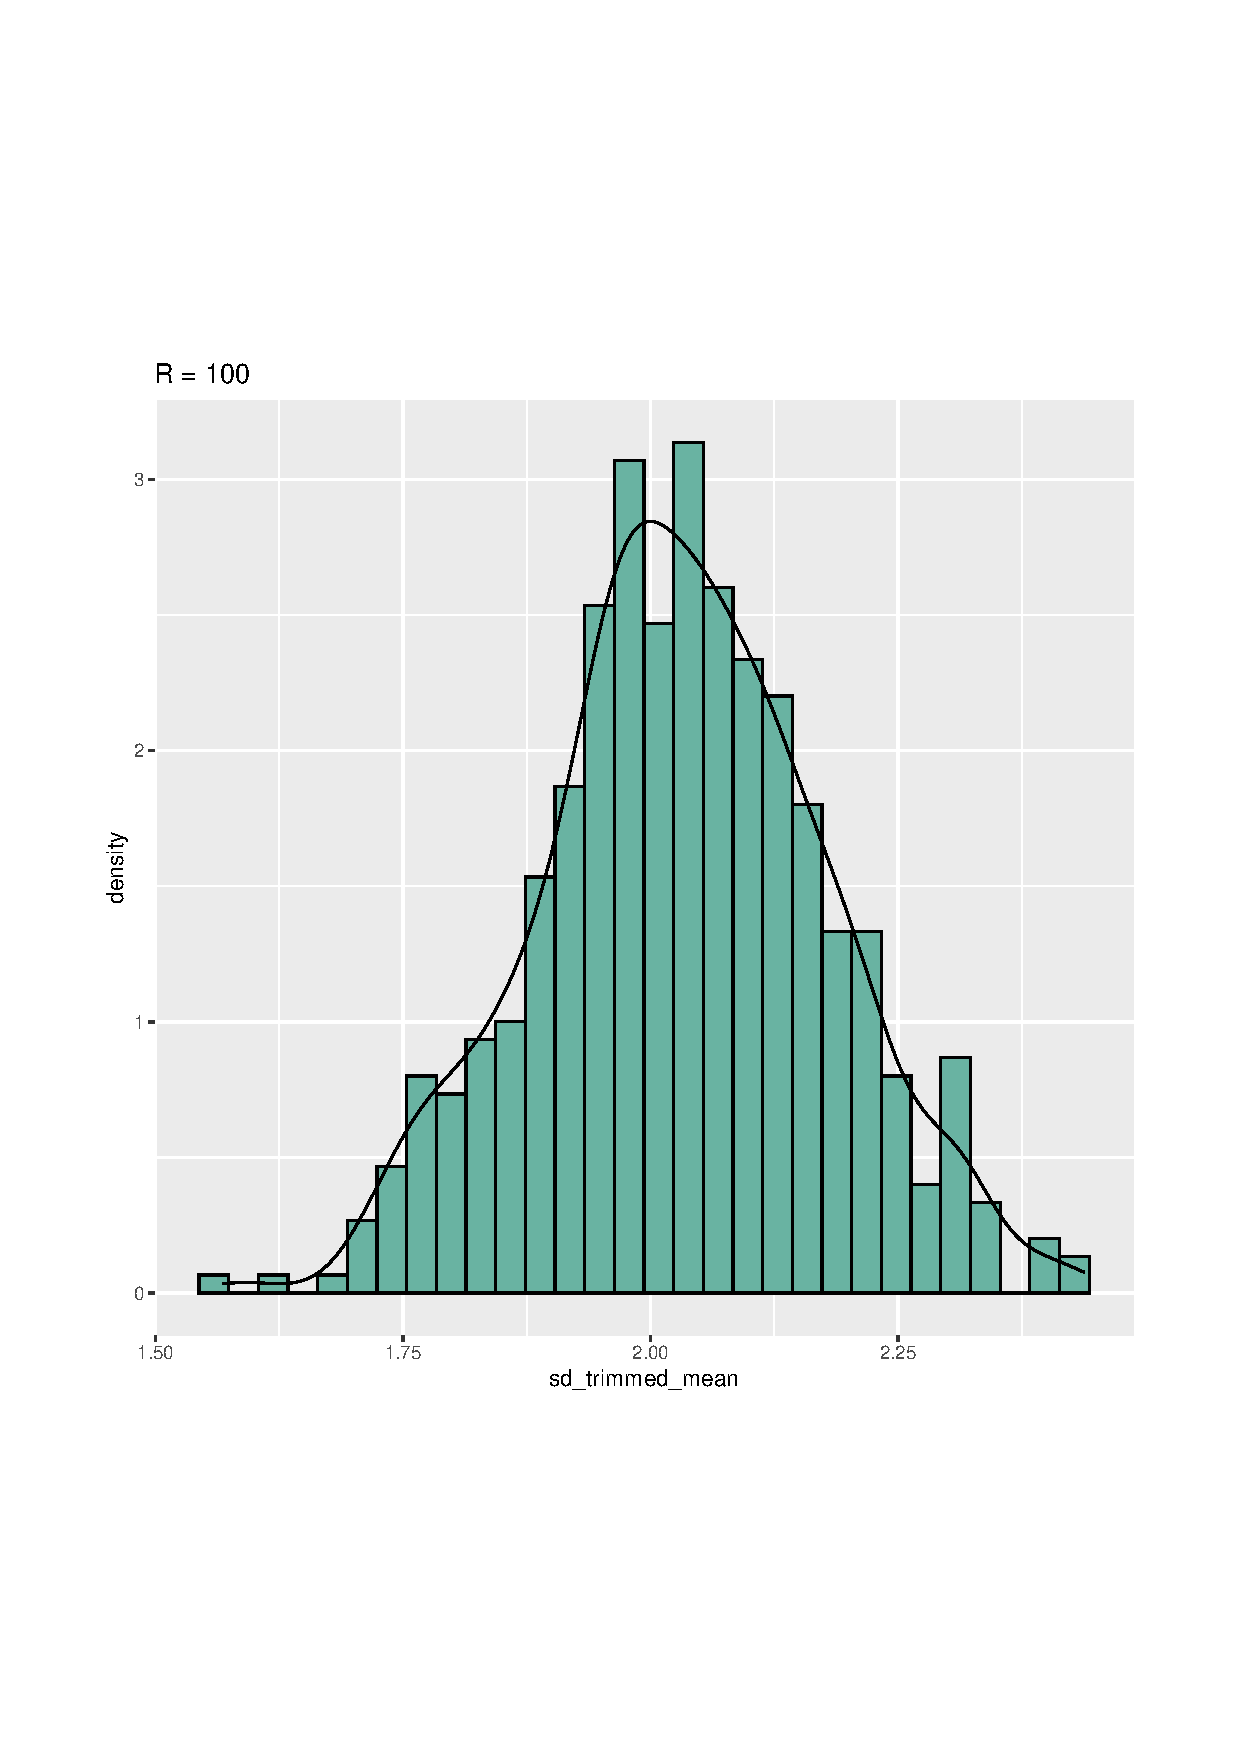
\includegraphics[width=.45\textwidth]{img/fig2}
}

\vspace{-10em}

\subfigure{
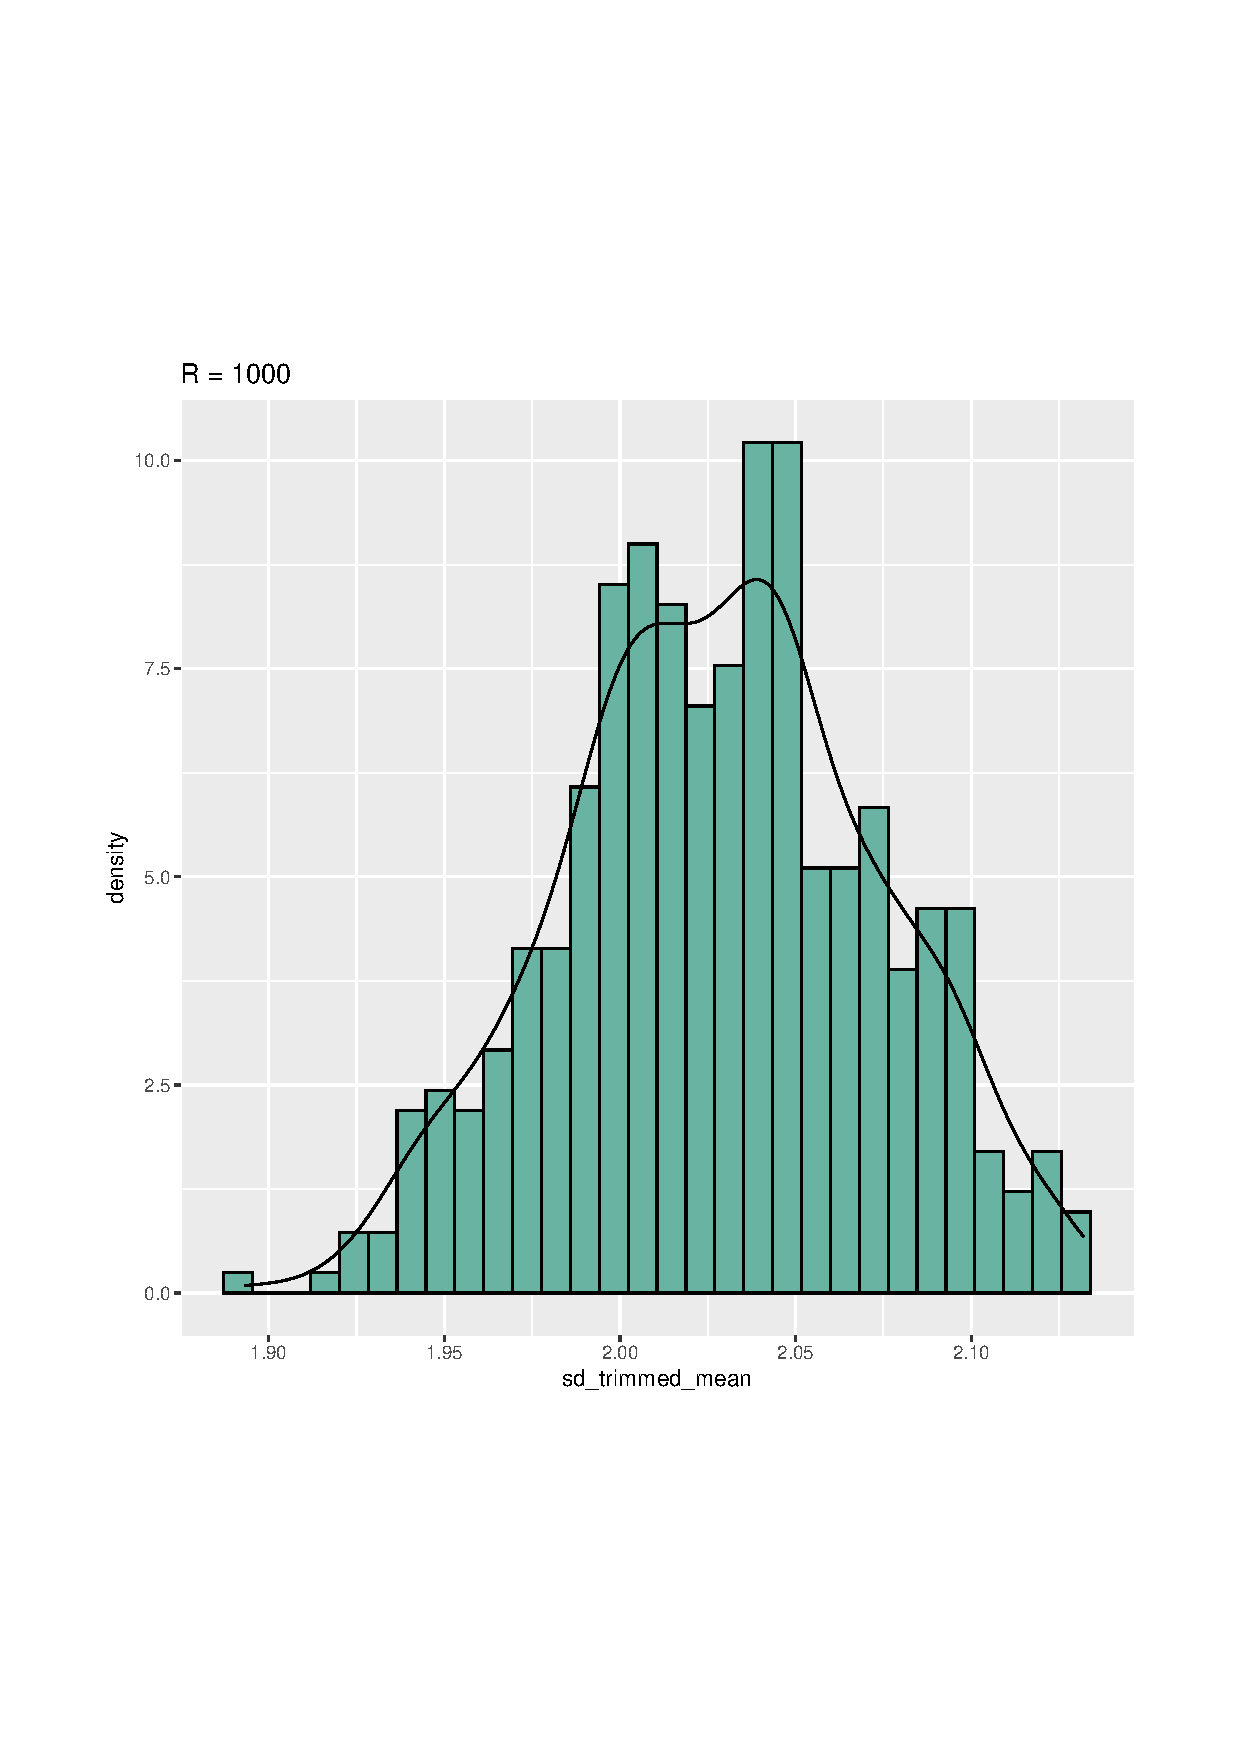
\includegraphics[width=.45\textwidth]{img/fig3}
}
\subfigure{
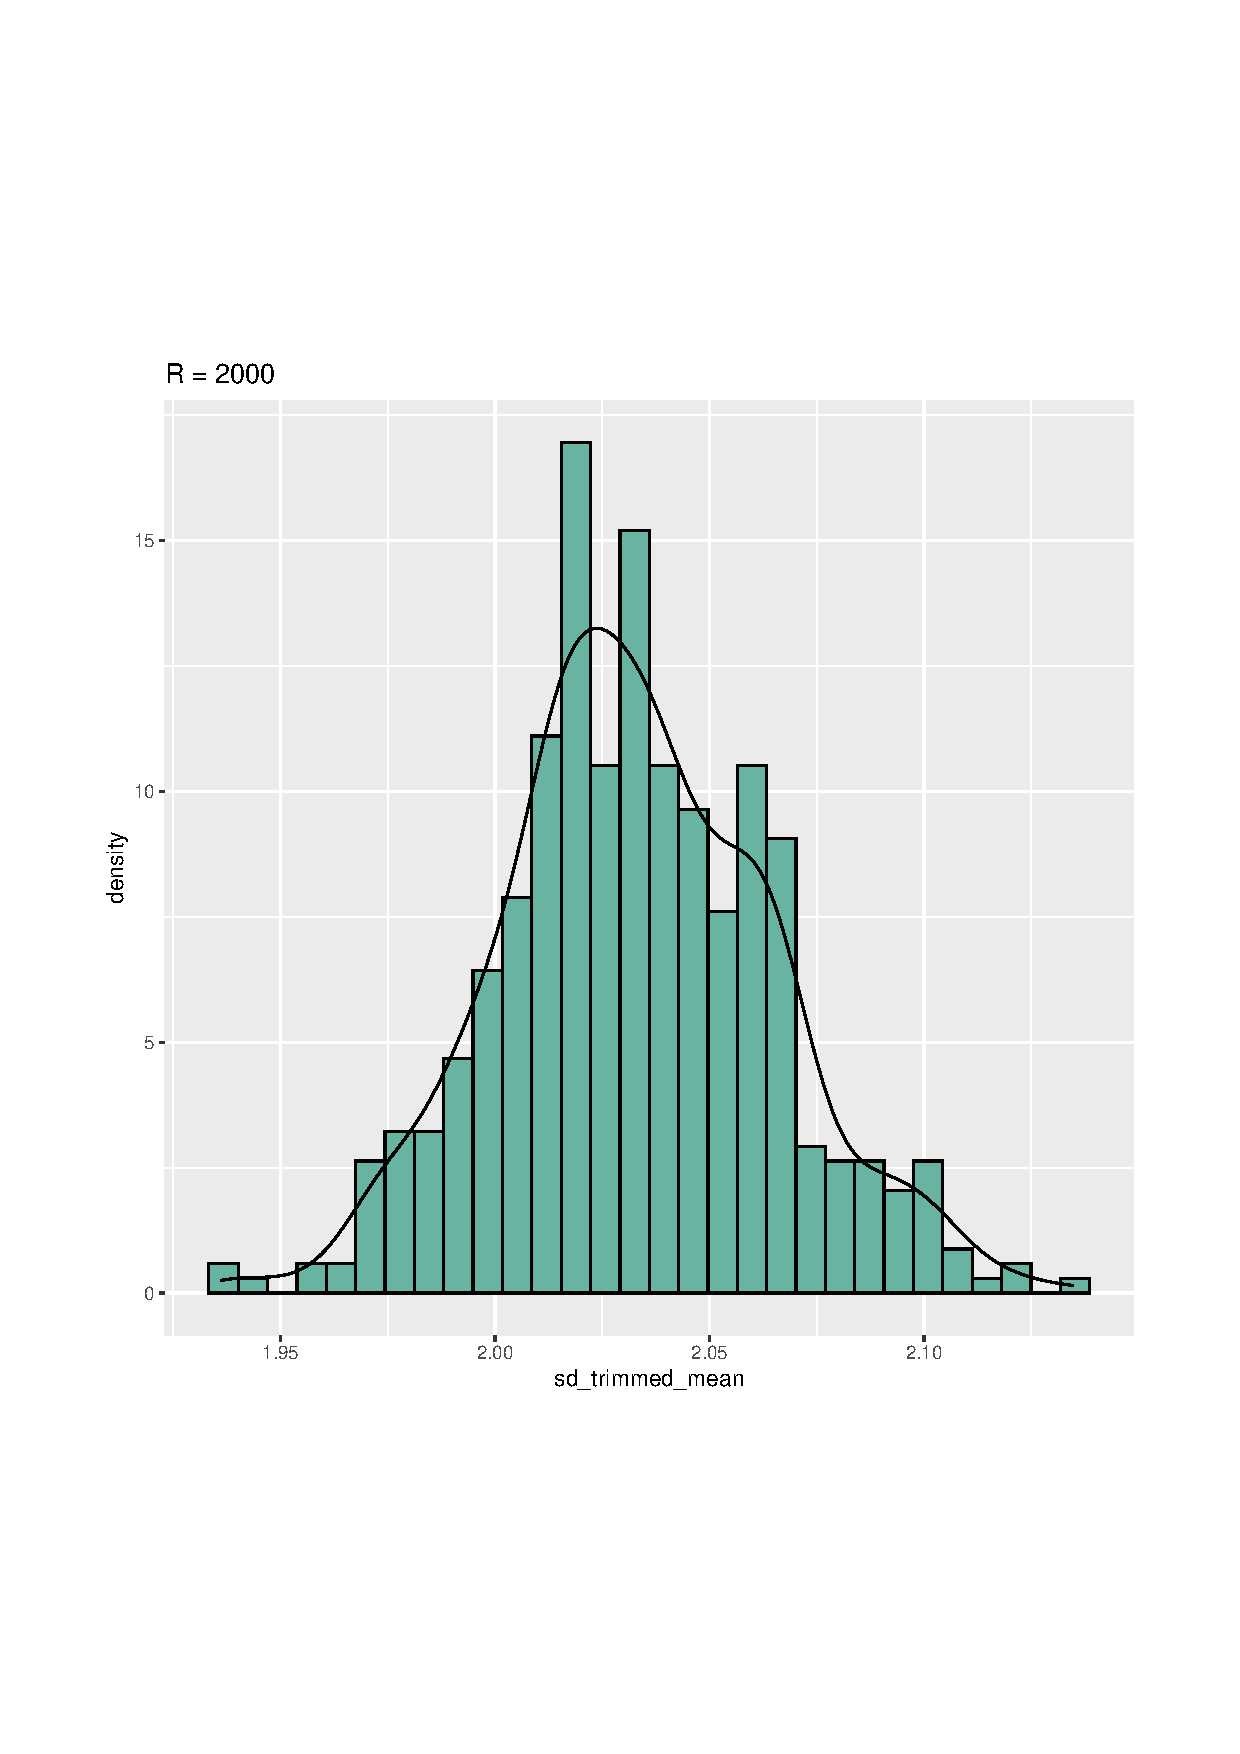
\includegraphics[width=.45\textwidth]{img/fig4}
}
\vspace{-4.5em}
  \caption{Histogramas y densidad estimada de $\hat\sigma_R$ con 500 repeticiones independientes, para distintos valores de $R$.}
\end{figure}

Podemos estimar teóricamente la desviación típica de la media de muchas repeticiones independientes del cálculo de $\hat\sigma_R$. Si tenemos $B$ estimaciones $\hat\sigma_R^{1}, \dots, \hat\sigma_R^{B}$, podemos calcular su media como

\[
\overline{\hat\sigma_R} = \frac{1}{B}\sum_{b=1}^B \hat\sigma_R^{b},
\]
y la varianza de esta media es entonces

\[
Var(\overline{\hat\sigma_R}) = \frac{Var(\hat\sigma_R^1)}{B}.
\]
Podemos estimar esta cantidad sustituyendo la varianza teórica de $\hat\sigma_R^1$ por la varianza muestral $S^2_B$ de la muestra $\hat\sigma_R^{1}, \dots, \hat\sigma_R^{B}$, llegando al estimador:

\begin{equation}
  \label{eq:est}
\widehat{Var(\overline{\hat\sigma_R})} = \frac{S^2_B}{B},
\end{equation}
y así el error típico estimado de la media de $B$ repeticiones independientes será la raíz cuadrada de \eqref{eq:est}.

\begin{minted}{R}
# Mean and standard error of the nrep estimators
cat("Mean of", nrep, "independent simulations ( R =", R, "):",
     mean(sd_trimmed_mean), "\n")
cat("Standard error:", sd(sd_trimmed_mean)/sqrt(nrep), "\n")
\end{minted}
Por ejemplo, los valores para el caso $R=100$ son $2.0332 \pm 0.0064$ y para el caso $R=1000$ son $2.0283 \pm 002$, donde vemos que el error típico es ya bastante pequeño.

\begin{ejer}
Sea $S^2$ la varianza muestral de una muestra de vaiid $X_1,\dots, X_n$ de una distribución con varianza $\sigma^2$. Podemos incluir en nuestro programa el cálculo de este valor:

\begin{enumerate}
  \item[a)] Para la muestra del problema anterior se tiene $S^2\approx 30.8423$. Usa bootstrap para determinar el error típico de este estimador de $\sigma^2$.
  \item[b)] Compara el resultado con el error típico que darías si, por ejemplo, supieras que los datos proceden de una distribución normal.
  \item[c)] Calcula un intervalo de confianza para $\sigma^2$ usando el método de bootstrap híbrido. Fija $1-\alpha=0.95$.
\end{enumerate}
\end{ejer}

\textit{Solución}. Para el apartado $a)$ queremos estimar el error típico del estimador $\hat\theta =S^2$ de la varianza $\theta=\sigma^2$. El enfoque es muy similar al del ejercicio anterior: el estimador bootstrap $\hat\sigma_R$ será el que viene dado por la raíz cuadrada de la expresión \eqref{eq:bootstrap}, donde ahora tendremos

\[
\hat\theta_j^* = \frac{1}{n-1} \sum_{i=1}^n \left( X_i^{*j} - \bar{X}^{*j}\right)^2.
\]
Modificamos ligeramente el programa que hicimos para incluir estos cambios:

\begin{minted}{R}
library(ggplot2)
set.seed(42)

# Parameters
R <- 1000
n <- 10

# Original sample
sample_orig <- c(1,2,3.5,4,7,7.3,8.6,12.4,13.8,18.1)
var_orig <- var(sample_orig)

# Bootstrap resamples (n x R matrix, one resample for each column)
resample_bootstrap <- sample(sample_orig, n*R, rep = T)
resample_bootstrap <- matrix(resample_bootstrap, nrow = n)

# Variance of the bootstrap resamples
var_bootstrap <- apply(resample_bootstrap, 2, var)

# Histogram of bootstrap variances
df <- data.frame(var_bootstrap = var_bootstrap)
ggplot(df, aes(x = var_bootstrap)) +
  geom_histogram(aes(y = ..density..),
                 bins = 20, fill = "#69b3a2", col = 'black') +
  geom_vline(xintercept = var_orig, size = 1.1, col ='red') +
  geom_density(aes(y=..density..))

# Bootstrap estimate of the sd of the variance
sd_var <- sd(var_bootstrap)
cat("Bootstrap estimate:", sd_var, "\n")
\end{minted}

Tras ejecutarlo con $R=1000$ remuestras, obtenemos como resultado una estimación de $\hat\sigma_R=10.6854$. Podemos ver en la siguiente figura un histograma con los valores de las varianzas de las remuestras para observar gráficamente su dispersión.

\begin{figure}[h!]
  \centering
  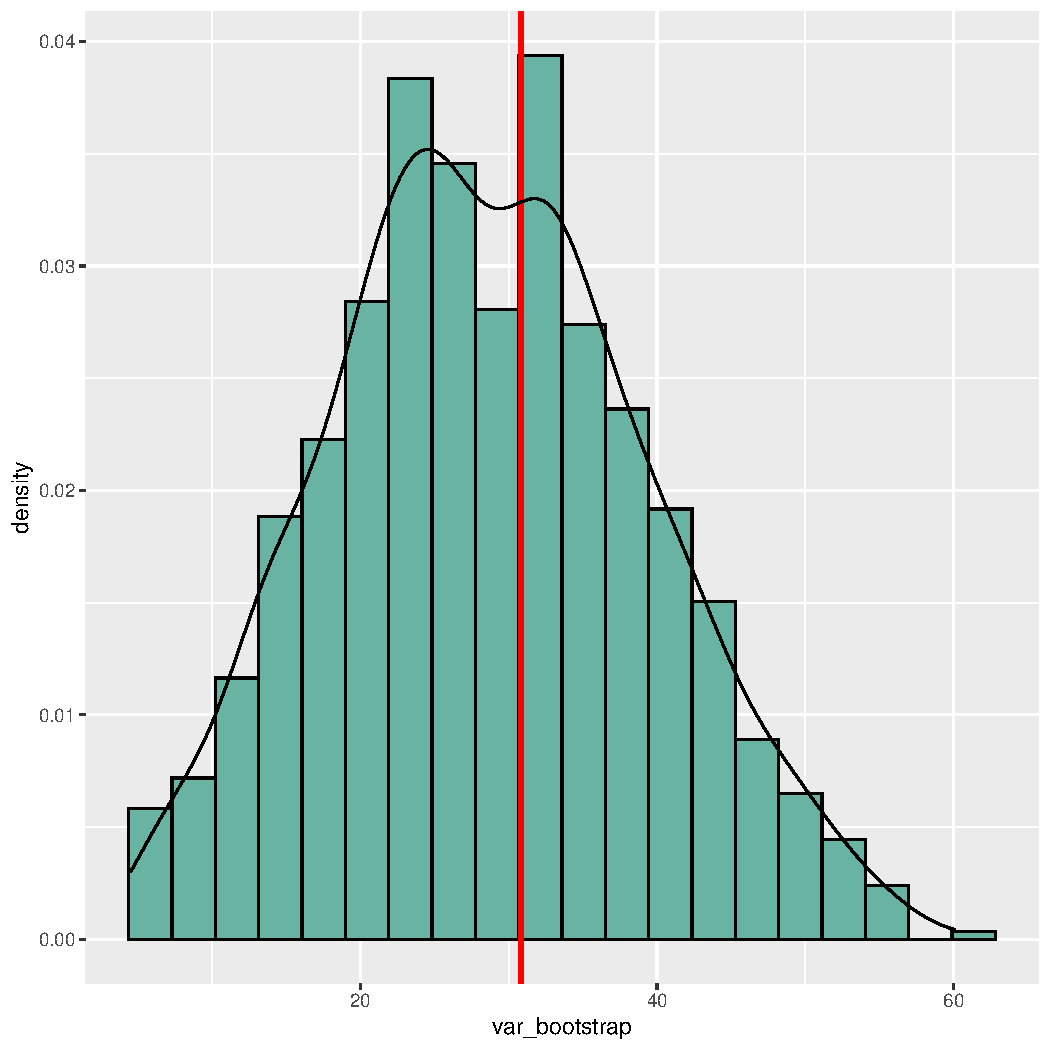
\includegraphics[width=0.5\linewidth]{img/fig5}
  \caption{Varianza de las 1000 remuestras bootstrap.}
\end{figure}

Para el apartado $b)$, conviene recordar que para una muestra de vaiid normales con varianza $\sigma^2$, se tiene que

\[
\frac{(n-1)S^2}{\sigma^2} \sim \chi^2_{n-1}.
\]
Tomando varianzas a ambos lados tenemos que

\[
\frac{(n-1)^2}{\sigma^4}Var(S^2)=2(n-1),
\]
luego despejando,

\[
Var(S^2)=\frac{2\sigma^4}{n-1}.
\]
El estimador natural de $Var(S^2)$ sería entonces

\[
\widehat{Var}(S^2)=\frac{2S^4}{n-1},
\]
y el estimador $\hat\sigma_{S^2}$ de la desviación típica de $S^2$ sería la raíz cuadrada de $\widehat{Var}(S^2)$. En nuestro caso $n=10$ y $S^2\approx 30.8423$, luego la estimación que daríamos sería

\[
\hat\sigma_{S^2}=\sqrt{\frac{2(30.8423)^2}{9}} \approx 14.5392.
\]

Finalmente, pasamos a resolver el apartado $c)$, donde nos piden calcular un intervalo de confianza para $\sigma^2$ usando el método de bootstrap híbrido. Definimos el estadístico

\[
T(X_1,\dots,X_n; F)=\sqrt{n}(S_n^2 - \sigma^2),
\]
y sabemos que si su distribución $H_n(x)$ fuera conocida, podríamos obtener un intervalo de confianza a nivel $1-\alpha$ como:

\[
(S^2 - n^{-1/2}H_n^{-1}(1-\alpha/2), \ S^2 - n^{-1/2}H_n^{-1}(\alpha/2)).
\]

Como la distribución de $H_n$ no es conocida, resulta natural sustituir su valor por el del estimador bootstrap $\hat H_n$, o más concretamente, por la aproximación con $R$ remuestras del mismo. De esta forma realizamos $R$ remuestreos bootstrap, para cada remuestra $b$ calculamos el valor de $T^{*b}=\sqrt{n}((S^2)^{*b} - S^2)$, los ordenamos, y seleccionamos los percentiles que dejan una proporción de valores $\alpha/2$ a derecha e izquierda. Estos valores son los que usamos en lugar de $H_n^{-1}(1-\alpha/2)$ y $H_n^{-1}(\alpha/2)$. Para implementar este procedimiento escribimos un pequeño programa, que detallamos a continuación.

\begin{minted}{R}
set.seed(42)

# Parameters
R <- 1000
n <- 10
alpha <- 0.05

# Original sample
sample_orig <- c(1,2,3.5,4,7,7.3,8.6,12.4,13.8,18.1)
var_orig <- var(sample_orig)

# Bootstrap resamples (n x R matrix, one resample for each column)
resample_bootstrap <- sample(sample_orig, n * R, rep = T)
resample_bootstrap <- matrix(resample_bootstrap, nrow = n)

# Variance of the bootstrap resamples
var_bootstrap <- apply(resample_bootstrap, 2, var)

# Bootstrap estimator T*
T_bootstrap <- sqrt(n) * (var_bootstrap - var_orig)

# Get limits of the confidence interval
ci_left <- var_orig - quantile(T_bootstrap, 1 - alpha/2)/sqrt(n)
ci_right <- var_orig - quantile(T_bootstrap, alpha/2)/sqrt(n)

cat("Confidence interval for sigma²: (", ci_left, ",", ci_right, ")\n")
\end{minted}

Vemos que el intervalo de confianza obtenido es $(11.3153, 52.8973)$, es decir, según nuestra estimación bootstrap se tiene que:

\[
P(11.3153 < \sigma^2 < 52.8973) = 0.95.
\]


\end{document}
